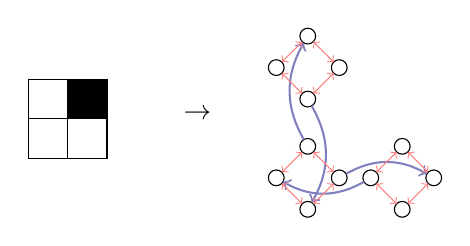
\begin{tikzpicture}
      \tikzstyle{bordered} = [draw,outer sep=0,inner sep=1,minimum size=0.5cm]
      \tikzstyle{state} = [draw,circle,outer sep=0,inner sep=1,minimum size=0.2cm]
      \tikzstyle{move}=[->,bend left,line width=0.75pt,blue!50!black!50]
      \tikzstyle{turn}=[<->,red!50]
	\node [bordered] at (-0.5,0) {};
\node [bordered,fill] at (0,0) {};
\node [bordered] at (-0.5,-0.5) {};
\node [bordered] at (0,-0.5) {};
\node [state] (v9) at (2.4,0.4) {};
\node [state] (v4) at (2.8,0.8) {};
\node [state] (v10) at (3.2,0.4) {};
\node [state] (v1) at (2.8,0) {};
\node [state] (v3) at (2.8,-0.6) {};
\node [state] (v8) at (2.4,-1) {};
\node [state] (v2) at (2.8,-1.4) {};
\node [state] (v5) at (3.2,-1) {};
\node [state] (v7) at (3.6,-1) {};
\node [state] (v11) at (4,-0.6) {};
\node [state] (v6) at (4.4,-1) {};
\node [state] (v12) at (4,-1.4) {};
\draw [move] (v1) edge (v2);
\draw [move] (v3) edge (v4);
\draw [move] (v5) edge (v6);
\draw [move] (v7) edge (v8);
\draw [turn] (v4) edge (v9);
\draw [turn] (v9) edge (v1);
\draw [turn] (v1) edge (v10);
\draw [turn] (v10) edge (v4);
\draw [turn] (v3) edge (v8);
\draw [turn] (v8) edge (v2);
\draw [turn] (v2) edge (v5);
\draw [turn] (v5) edge (v3);
\draw [turn] (v7) edge (v11);
\draw [turn] (v11) edge (v6);
\draw [turn] (v12) edge (v6);
\draw [turn] (v12) edge (v7);
\node at (1.4,-0.2) {$\rightarrow$};
\end{tikzpicture}